\documentclass[12pt]{article}
\usepackage{fullpage}
\usepackage{lscape}
\usepackage[top=2cm, bottom=4.5cm, left=2.5cm, right=2.5cm]{geometry}
\usepackage{amsmath,amsthm,amsfonts,amssymb,amscd}
\usepackage{lastpage}
\usepackage{enumerate}
\usepackage{fancyhdr}
\usepackage{mathrsfs}
\usepackage{xcolor}
\usepackage{graphicx}
\usepackage{subcaption}
\usepackage{listings}
\usepackage{hyperref}
\usepackage{titlesec}

\setcounter{secnumdepth}{4}
\titleformat{\paragraph}
{\normalfont\normalsize\bfseries}{\theparagraph}{1em}{}
\titlespacing*{\paragraph}
{0pt}{3.25ex plus 1ex minus .2ex}{1.5ex plus .2ex}

\hypersetup{%
  colorlinks=true,
  linkcolor=blue,
  linkbordercolor={0 0 1}
}

\lstdefinestyle{C++}{
    language        = C++,
    frame           = lines, 
    basicstyle      = \footnotesize,
    keywordstyle    = \color{blue},
    stringstyle     = \color{olive},
    commentstyle    = \color{red}\ttfamily,
    breaklines      = true,
    tabsize         = 2
}

\setlength{\parindent}{0.0in}
\setlength{\parskip}{0.05in}

\newcommand\code{\url}
\newcommand\course{COMP0023}
\newcommand\hwnumber{}                   
\newcommand\NetIDa{17134402}            \newcommand\NetIDb{-}            
\pagestyle{fancyplain}
\headheight 35pt
\lhead{\NetIDa}
\lhead{\NetIDa\\\NetIDb}                 
\chead{\textbf{\Large Assessment \hwnumber}}
\rhead{\course \\ \today}
\lfoot{}
\cfoot{}
\rfoot{\small\thepage}
\headsep 1.5em

\graphicspath{{./images/}}

\begin{document}

\section{}

\subsection{Single Packet Perspective}

With regards to any bit errors or packet corruptions, each network layer will have their separate effort to detect and correct error.

\subsubsection{Physical Layer L1}

Errors are detected on the link via Error Control Coding (ECC), and can potentially further corrected by Forward Error Correction (FEC) methods. 

As of ECC, slower Ethernet specifications (Fast Ethernet, and Gigabit Ethernet), have limited error detection methods. For example, 8b/10b encoding used in Gigabit Ethernet does allow detecting single-bit errors, but not correcting them. 

Later developments of faster Ethernet specifications includes ECC methods and even optional FEC sublayer. Take IEEE 802.3ap for example, 10GBASE-R PHYs uses the 64b/66b encoding which provides at least a 4-bit hamming distance protection for all packet data. Moreover, Clause 74 specifies an optional RS-FEC(2112, 2080) sublayer using the Reed–Solomon error correction algorithm for 10GBASE-R PHYs. It is in essence a shortented cyclic code with 32 parity bits, appended to 32 64-bit payload words (65-bit actual payload), hence the $32*(64 + 1) + 32 = 2112$.

Furthermore, higher symbol rate PHY links have much stronger FEC methods in place. IEEE 802.3bj describing 100G backplane PHY links deems FEC mandatory in its higher bit rate or longer distance connections.

In all, at a PHY level, a packet with minimal bit errors on a link with FEC can potentially be corrected. If no FEC is in-place, or larger and longer burst errors happened on the link, the PHY might deem certain received encoding invalid and discard the packet altogether.

\subsubsection{Link Layer L2}

On the link layer, most notably the Ethernet II, employs a Frame Check Sequence (FCS) appending to the end of the packet before the interframe gap. The FCS is calculated using a 32-bit cyclic-redundancy-check (CRC32) algorithm, transmitting in little-endian bit order. CRC32 is a powerful algorithm that detects:
\begin{itemize}
    \item All burst errors of length $<= 31$
    \item All odd number of bit errors
    \item With high probability, burst errors of length $>= 32$
\end{itemize}

Although there are several research regarding using CRC to do error correction, it is still rare and we can reasonably assume that a faulty Ethernet frame detected by CRC32 would be dropped.

\subsubsection{Network Layer L3 and Transport Layer L4}

In the case of Internet Protocol version 4 (IPv4), its checksum is a one's complement checksum operating upon the IP header only. The primary purpose of which is to ensure correctness in a multi-host and multi-hop environment. The IP checksum is aimed at detecting errors in L3 switches and intermediate machines, as they could potentially alter the IP header during an Internet packet transmission.

TCP checksum is also a one's complement checksum. It is enforced upon several fields, including the TCP header, the TCP payload, and an IP pseudo-header. The IP pseudo-header includes the src and dst IP, TCP's protocol number $\mathtt{0x06}$, as well as the IP size field extracted from the lower level. This checksum is meant to be an End-to-End (E2E) verification of the packet's integrity.

UDP checksum is not mandatory upon UDP/IPv4 stack. Similarly with TCP checksum, UDP checksum is also a 1's complement of the header, payload and an IP pseudo-header, as elaborated above.

Contrary to IPv4, IPv6 does not have a checksum field. On a good note, this saves routers' time as they do not have to recalculate checksum to upon forwarding packets. The designers believe that L2 CRC checksum and mandatory L4 checksum would bring sufficient ECC to the L3 header. Thus, UDP checksum is mandatory for UDP/IPv6.

One's complement checksum is not particularly powerful as they only guarantees single-bit error detection. However, it's primarily designed to work in an CPU-efficient (calculated in bytes) and space efficient (16 bits for any message length) way.

In both ways, if the one's complement detects an error, the packet would most likely be dropped. In the rare case where the error is not detected in L1-L4, the erroneous packet would be sent to the upper layer.

\subsubsection{Summary}

In conclusion, the corrupted packet, if not severe, can be potentially corrected on the PHY link given FEC is in-place. If not, or if there is error detected on L2, L3 and L4, the packet would be discarded. In the worst case that the corrupted bits are ordered in a particular way that escapes ECC in all 4 layers, the packet will be passed on to the destination host's application.

\subsection{End-To-End Perspective}

In the following discussions, we will divide the each section into whether the corrupted bit is detected or not in the ECCs of L1-L4.

\subsubsection{DNS transactions}

Upon typing the URL \url{www.ucl.ac.uk} into the browser, the laptop would first query the DNS to obtain the URL's IP address. For the sake of simplicity, we assume the domain operates with DNS instead of DNSSEC. However, DNSSEC verifies the message authenticity and the bit corruptions would impact its payload in roughly the same way as DNS.

\begin{itemize}
    \item Laptop looks up the DNS information of the URL in cache, since it's a new one, it would not be found
    \item Laptop sends a DNS request to the configured DNS server, usually a local DNS resolver, a public DNS resolver, or a ISP DNS resolver
    \item If found, the DNS reply containing \url{www.ucl.ac.uk}'s IP address would be replied to the laptop
    \item If not found, the DNS resolver would start resolving \url{www.ucl.ac.uk} from the root servers, all the way down to the authoritative nameservers (i.e. \url{dns-ns1.ucl.ac.uk}).
    \item Similarly, a DNS reply of \url{www.ucl.ac.uk} would be responded to the laptop.
\end{itemize}

\paragraph{Packet Error Detected}

In this process, as suggested, the packet would most likely be discarded by a switch, router or server upon corruption. Then, the laptop browser would timeout on the DNS query and re-send it after a while. 

\paragraph{Packet Error Not Detected}

In the rare case where the bits corrupted evades all the checksums measures, resulting in either an invalid DNS query, or a DNS query targetting a different domain. The common case would be an invalid DNS query, for example an invalid Flags field. The name server or resolver shall detect this and drop this invalid DNS query. The rarer case would be the request reaching a entirely different authoritative server, and getting either a \url{NXDOMAIN} reply or a reply about different domain (i.e. \url{www.ual.ac.uk}). The laptop would found the reply not related to its question. Hence, re-querying the DNS of \url{www.ucl.ac.uk}.

\subsubsection{HTTP transactions}

Generally speaking, \url{www.ucl.ac.uk} being visited in a laptop browser shall be HTTP webpages (certainly not Gopher). Although UCL's HTTP server only operates on HTTP/1.1, \url{www.ucl.ac.uk/} webpage also includes content served by Cloudlflare's CDN through HTTP/3, optionally. It's notable that visiting a webpage through HTTP/3 is based on QUIC/UDP/IP stack, while HTTP/1.1 is based on a TCP/IP stack. In this question, we limit the scope to HTTP/(TLS)/TCP/IP stack. However, QUIC/UDP is generally comparable to TCP/IP and the analysis shall be largely similar. Also, we will make an reasonable assumption of using HTTP in this case (not secure).

\paragraph{Packet Error Detected}

The TCP connection establishment is comprised of three handshakes. In the case where the laptop's packet corrupted on the first SYN or the third ACK, the server would just not proceed, until the RTX timer runs out on the laptop and resends a SYN or ACK respectively.

During the transmission process, if any of the laptop's packet is corrupted in the middle, the RTX timer could just simply timeout as the corresponding ACK will not be received. Thus, the laptop would attempt to retransmit until successful.

The TCP connection tear down is comprised of four handshakes. In the case where the first FIN from laptop gets corrupted, the server would not know the attempt to tear down connection, and surely would not reply with an ACK. After the RTX timeout, the laptop would re-attempt to transmit the FIN packet.

The special case lies in the corruption of the fourth ACK (corresponding to server FIN) from the laptop. At this time, the laptop would have entered a TIME\_WAIT state, expecting to close the connection after 2 Maximum Segment Lifetimes (MSLs). However, the server, not knowing its FIN is ACKed by the laptop but lost due to bit corruptions, would eventually reach RTX timeout. The server would retransmit a FIN to the laptop, which shall reach the laptop during TIME\_WAIT. The laptop will then retransmit the corrupted ACK to the server and successfully close the connection.

\paragraph{Packet Error Not Detected}

In the rare case where the packet error is not detected, the serving application might receive a corrupted request. Typically, the HTTP request would be an invalid one. In the extreme case where the corrupted HTTP request is valid, and contains a different URL, the server might respond with a HTTP error code (404), or with a different webpage as specified in the corrupted packet. The server behaviour would be unpredictable in this case.


\section{}

\renewcommand{\thesubsection}{\thesection.\alph{subsection}}

\subsection{}

\begin{figure}[h!]
  \makebox[\textwidth][c]{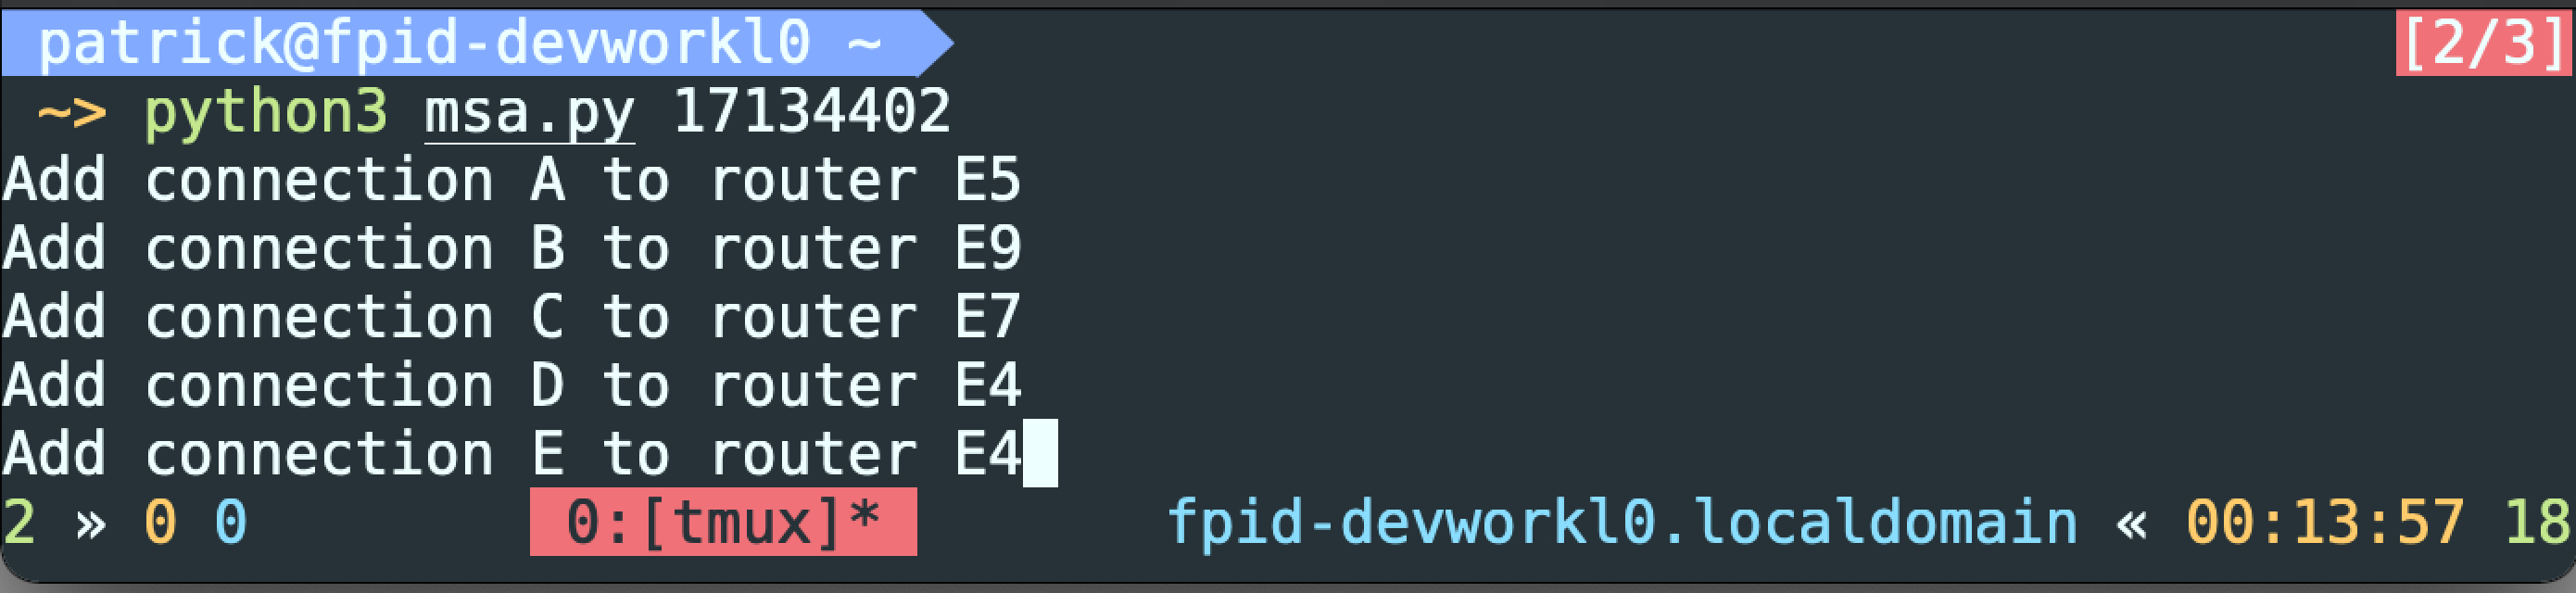
\includegraphics[width=\textwidth]{imgs/python-script-screenshot.png}}
  \caption{Python Script Screenshot}
  \label{fig:python-screenshot}
\end{figure}

\begin{figure}[h!]
  \makebox[\textwidth][c]{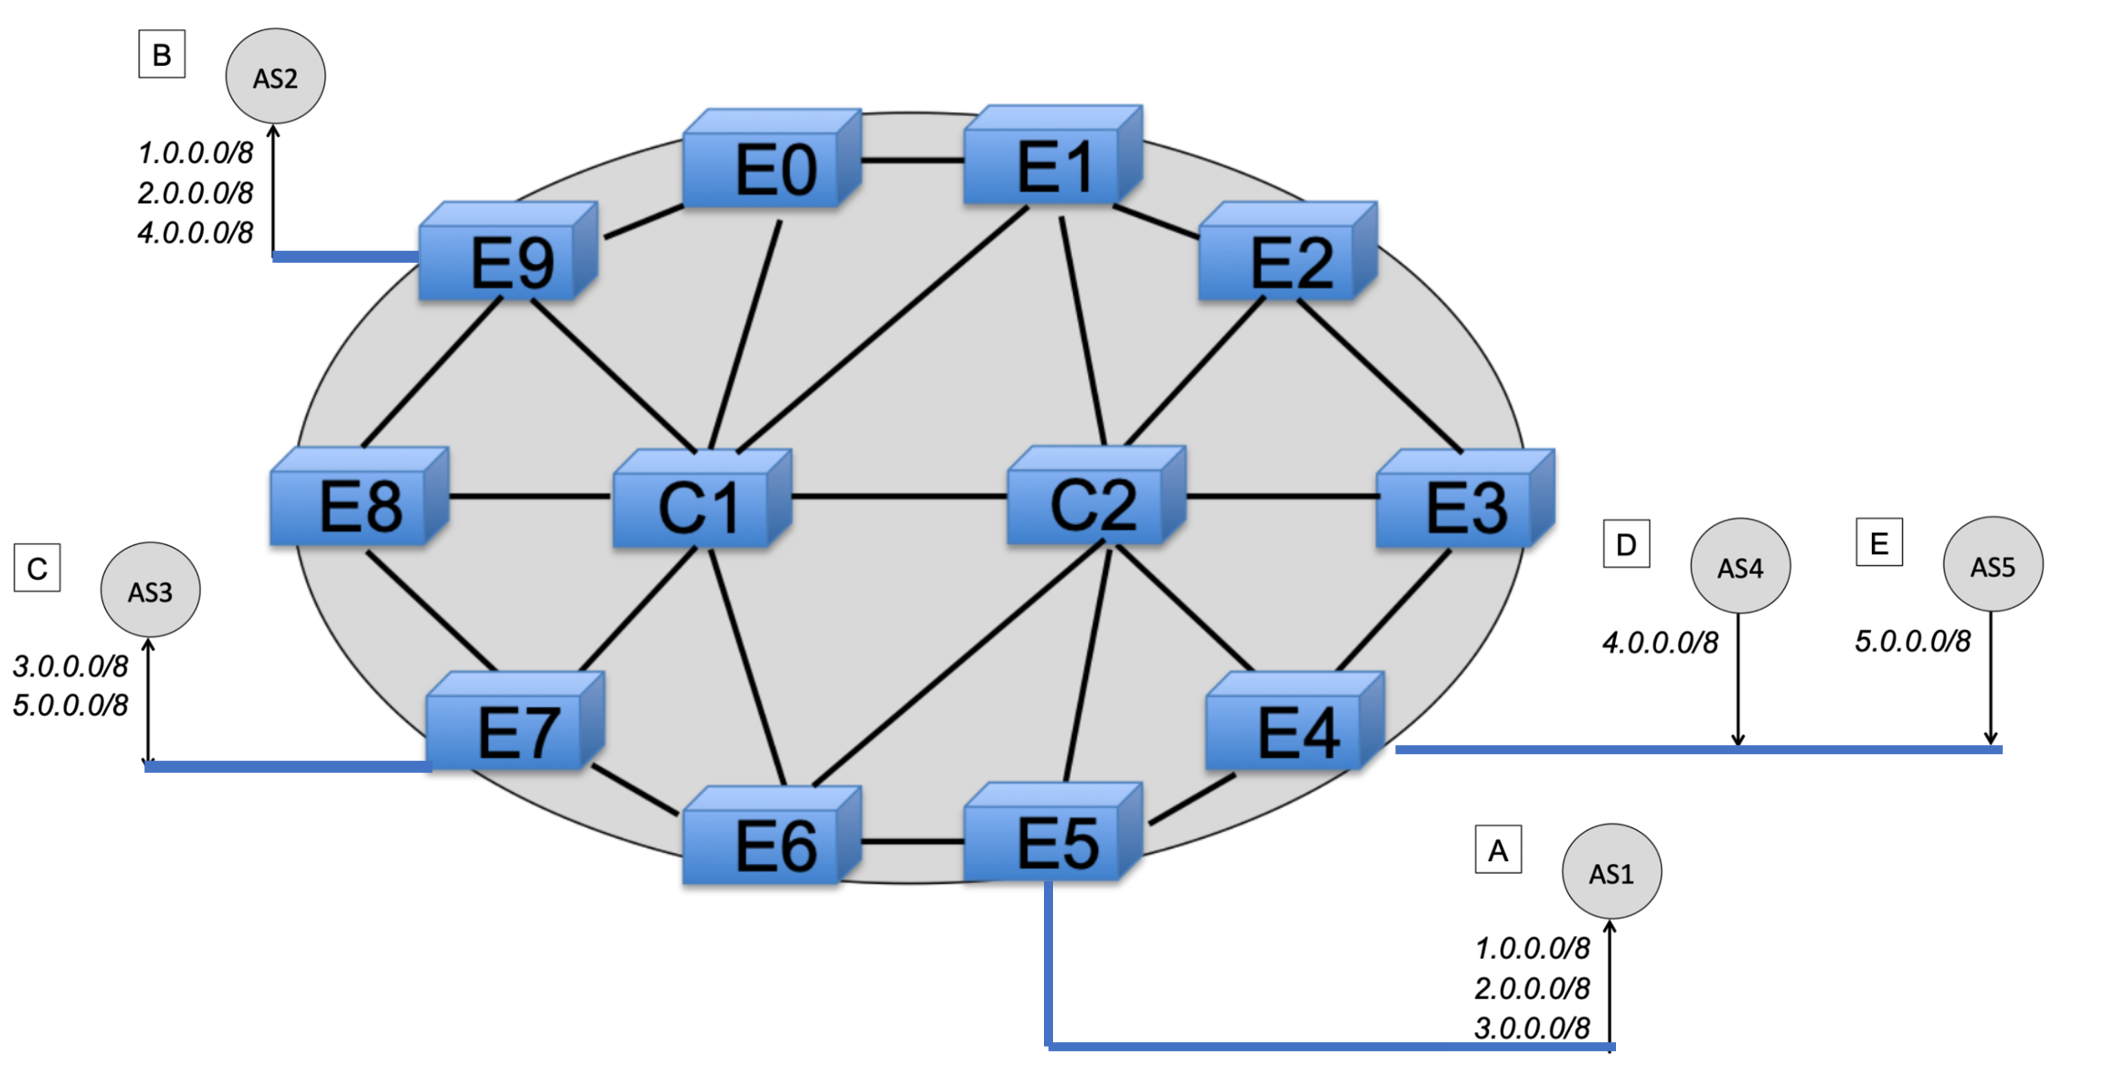
\includegraphics[width=1.1\textwidth]{imgs/topology.png}}
  \caption{Topology}
  \label{fig:topology}
\end{figure}

\subsection{}




\end{document}